\documentclass[12pt,a4paper]{article}

\usepackage[a4paper,text={16.5cm,25.2cm},centering]{geometry}
\usepackage{lmodern}
\usepackage{amssymb,amsmath}
\usepackage{graphicx}
\usepackage{microtype}
\usepackage{hyperref}
\setlength{\parindent}{0pt}
\setlength{\parskip}{1.2ex}

\hypersetup
       {   pdfauthor = { Chris Rackauckas },
           pdftitle={ Linear 100x100 Work-Precision Diagrams },
           colorlinks=TRUE,
           linkcolor=black,
           citecolor=blue,
           urlcolor=blue
       }

\title{ Linear 100x100 Work-Precision Diagrams }

\author{ Chris Rackauckas }


\usepackage[T1]{fontenc}
\usepackage{textcomp}
\usepackage{upquote}
\usepackage{listings}
\usepackage{xcolor}
\lstset{
    basicstyle=\ttfamily\footnotesize,
    upquote=true,
    breaklines=true,
    keepspaces=true,
    showspaces=false,
    columns=fullflexible,
    showtabs=false,
    showstringspaces=false,
    escapeinside={(*@}{@*)},
    extendedchars=true,
}
\newcommand{\HLJLt}[1]{#1}
\newcommand{\HLJLw}[1]{#1}
\newcommand{\HLJLe}[1]{#1}
\newcommand{\HLJLeB}[1]{#1}
\newcommand{\HLJLo}[1]{#1}
\newcommand{\HLJLk}[1]{\textcolor[RGB]{148,91,176}{\textbf{#1}}}
\newcommand{\HLJLkc}[1]{\textcolor[RGB]{59,151,46}{\textit{#1}}}
\newcommand{\HLJLkd}[1]{\textcolor[RGB]{214,102,97}{\textit{#1}}}
\newcommand{\HLJLkn}[1]{\textcolor[RGB]{148,91,176}{\textbf{#1}}}
\newcommand{\HLJLkp}[1]{\textcolor[RGB]{148,91,176}{\textbf{#1}}}
\newcommand{\HLJLkr}[1]{\textcolor[RGB]{148,91,176}{\textbf{#1}}}
\newcommand{\HLJLkt}[1]{\textcolor[RGB]{148,91,176}{\textbf{#1}}}
\newcommand{\HLJLn}[1]{#1}
\newcommand{\HLJLna}[1]{#1}
\newcommand{\HLJLnb}[1]{#1}
\newcommand{\HLJLnbp}[1]{#1}
\newcommand{\HLJLnc}[1]{#1}
\newcommand{\HLJLncB}[1]{#1}
\newcommand{\HLJLnd}[1]{\textcolor[RGB]{214,102,97}{#1}}
\newcommand{\HLJLne}[1]{#1}
\newcommand{\HLJLneB}[1]{#1}
\newcommand{\HLJLnf}[1]{\textcolor[RGB]{66,102,213}{#1}}
\newcommand{\HLJLnfm}[1]{\textcolor[RGB]{66,102,213}{#1}}
\newcommand{\HLJLnp}[1]{#1}
\newcommand{\HLJLnl}[1]{#1}
\newcommand{\HLJLnn}[1]{#1}
\newcommand{\HLJLno}[1]{#1}
\newcommand{\HLJLnt}[1]{#1}
\newcommand{\HLJLnv}[1]{#1}
\newcommand{\HLJLnvc}[1]{#1}
\newcommand{\HLJLnvg}[1]{#1}
\newcommand{\HLJLnvi}[1]{#1}
\newcommand{\HLJLnvm}[1]{#1}
\newcommand{\HLJLl}[1]{#1}
\newcommand{\HLJLld}[1]{\textcolor[RGB]{148,91,176}{\textit{#1}}}
\newcommand{\HLJLs}[1]{\textcolor[RGB]{201,61,57}{#1}}
\newcommand{\HLJLsa}[1]{\textcolor[RGB]{201,61,57}{#1}}
\newcommand{\HLJLsb}[1]{\textcolor[RGB]{201,61,57}{#1}}
\newcommand{\HLJLsc}[1]{\textcolor[RGB]{201,61,57}{#1}}
\newcommand{\HLJLsd}[1]{\textcolor[RGB]{201,61,57}{#1}}
\newcommand{\HLJLsdB}[1]{\textcolor[RGB]{201,61,57}{#1}}
\newcommand{\HLJLsdC}[1]{\textcolor[RGB]{201,61,57}{#1}}
\newcommand{\HLJLse}[1]{\textcolor[RGB]{59,151,46}{#1}}
\newcommand{\HLJLsh}[1]{\textcolor[RGB]{201,61,57}{#1}}
\newcommand{\HLJLsi}[1]{#1}
\newcommand{\HLJLso}[1]{\textcolor[RGB]{201,61,57}{#1}}
\newcommand{\HLJLsr}[1]{\textcolor[RGB]{201,61,57}{#1}}
\newcommand{\HLJLss}[1]{\textcolor[RGB]{201,61,57}{#1}}
\newcommand{\HLJLssB}[1]{\textcolor[RGB]{201,61,57}{#1}}
\newcommand{\HLJLnB}[1]{\textcolor[RGB]{59,151,46}{#1}}
\newcommand{\HLJLnbB}[1]{\textcolor[RGB]{59,151,46}{#1}}
\newcommand{\HLJLnfB}[1]{\textcolor[RGB]{59,151,46}{#1}}
\newcommand{\HLJLnh}[1]{\textcolor[RGB]{59,151,46}{#1}}
\newcommand{\HLJLni}[1]{\textcolor[RGB]{59,151,46}{#1}}
\newcommand{\HLJLnil}[1]{\textcolor[RGB]{59,151,46}{#1}}
\newcommand{\HLJLnoB}[1]{\textcolor[RGB]{59,151,46}{#1}}
\newcommand{\HLJLoB}[1]{\textcolor[RGB]{102,102,102}{\textbf{#1}}}
\newcommand{\HLJLow}[1]{\textcolor[RGB]{102,102,102}{\textbf{#1}}}
\newcommand{\HLJLp}[1]{#1}
\newcommand{\HLJLc}[1]{\textcolor[RGB]{153,153,119}{\textit{#1}}}
\newcommand{\HLJLch}[1]{\textcolor[RGB]{153,153,119}{\textit{#1}}}
\newcommand{\HLJLcm}[1]{\textcolor[RGB]{153,153,119}{\textit{#1}}}
\newcommand{\HLJLcp}[1]{\textcolor[RGB]{153,153,119}{\textit{#1}}}
\newcommand{\HLJLcpB}[1]{\textcolor[RGB]{153,153,119}{\textit{#1}}}
\newcommand{\HLJLcs}[1]{\textcolor[RGB]{153,153,119}{\textit{#1}}}
\newcommand{\HLJLcsB}[1]{\textcolor[RGB]{153,153,119}{\textit{#1}}}
\newcommand{\HLJLg}[1]{#1}
\newcommand{\HLJLgd}[1]{#1}
\newcommand{\HLJLge}[1]{#1}
\newcommand{\HLJLgeB}[1]{#1}
\newcommand{\HLJLgh}[1]{#1}
\newcommand{\HLJLgi}[1]{#1}
\newcommand{\HLJLgo}[1]{#1}
\newcommand{\HLJLgp}[1]{#1}
\newcommand{\HLJLgs}[1]{#1}
\newcommand{\HLJLgsB}[1]{#1}
\newcommand{\HLJLgt}[1]{#1}


\begin{document}

\maketitle

For these tests we will solve an 100x100 system of linear differential equations. This will demonstrate the efficiency of the methods for handling large systems. We will be mostly looking at the efficiency of the work-horse Dormand-Prince Order 4/5 Pairs: one from DifferentialEquations.jl (\texttt{DP5}, one from ODE.jl \texttt{rk45}, and one from ODEInterface: Hairer's famous \texttt{dopri5}).

Also included is \texttt{Tsit5}. While all other ODE programs have gone with the traditional choice of using the Dormand-Prince 4/5 pair as the default, DifferentialEquations.jl uses \texttt{Tsit5} as one of the default algorithms. It's a very new (2011) and not widely known, but the theory and the implimentation shows it's more efficient than DP5. Thus we include it just to show off how re-designing a library from the ground up in a language for rapid code and rapid development has its advantages.

\subsection{Setup}

\begin{lstlisting}
(*@\HLJLk{using}@*) (*@\HLJLn{DifferentialEquations}@*)(*@\HLJLp{,}@*) (*@\HLJLn{DiffEqDevTools}@*)(*@\HLJLp{,}@*) (*@\HLJLn{Plots}@*)(*@\HLJLp{,}@*) (*@\HLJLn{ODEInterfaceDiffEq}@*)(*@\HLJLp{,}@*) (*@\HLJLn{ODE}@*)
(*@\HLJLnf{gr}@*)(*@\HLJLp{()}@*)
(*@\HLJLcs{{\#} 2D Linear ODE}@*)
(*@\HLJLk{function}@*) (*@\HLJLnf{f}@*)(*@\HLJLp{(}@*)(*@\HLJLn{du}@*)(*@\HLJLp{,}@*)(*@\HLJLn{u}@*)(*@\HLJLp{,}@*)(*@\HLJLn{p}@*)(*@\HLJLp{,}@*)(*@\HLJLn{t}@*)(*@\HLJLp{)}@*)
  (*@\HLJLk{for}@*) (*@\HLJLn{i}@*) (*@\HLJLkp{in}@*) (*@\HLJLni{1}@*)(*@\HLJLoB{:}@*)(*@\HLJLnf{length}@*)(*@\HLJLp{(}@*)(*@\HLJLn{u}@*)(*@\HLJLp{)}@*)
    (*@\HLJLn{du}@*)(*@\HLJLp{[}@*)(*@\HLJLn{i}@*)(*@\HLJLp{]}@*) (*@\HLJLoB{=}@*) (*@\HLJLnfB{1.01}@*)(*@\HLJLoB{*}@*)(*@\HLJLn{u}@*)(*@\HLJLp{[}@*)(*@\HLJLn{i}@*)(*@\HLJLp{]}@*)
  (*@\HLJLk{end}@*)
(*@\HLJLk{end}@*)
(*@\HLJLk{function}@*) (*@\HLJLnf{f{\_}analytic}@*)(*@\HLJLp{(}@*)(*@\HLJLn{u\ensuremath{\_0}}@*)(*@\HLJLp{,}@*)(*@\HLJLn{p}@*)(*@\HLJLp{,}@*)(*@\HLJLn{t}@*)(*@\HLJLp{)}@*)
  (*@\HLJLn{u\ensuremath{\_0}}@*)(*@\HLJLoB{*}@*)(*@\HLJLnf{exp}@*)(*@\HLJLp{(}@*)(*@\HLJLnfB{1.01}@*)(*@\HLJLoB{*}@*)(*@\HLJLn{t}@*)(*@\HLJLp{)}@*)
(*@\HLJLk{end}@*)
(*@\HLJLn{tspan}@*) (*@\HLJLoB{=}@*) (*@\HLJLp{(}@*)(*@\HLJLnfB{0.0}@*)(*@\HLJLp{,}@*)(*@\HLJLnfB{10.0}@*)(*@\HLJLp{)}@*)
(*@\HLJLn{prob}@*) (*@\HLJLoB{=}@*) (*@\HLJLnf{ODEProblem}@*)(*@\HLJLp{(}@*)(*@\HLJLnf{ODEFunction}@*)(*@\HLJLp{(}@*)(*@\HLJLn{f}@*)(*@\HLJLp{,}@*)(*@\HLJLn{analytic}@*)(*@\HLJLoB{=}@*)(*@\HLJLn{f{\_}analytic}@*)(*@\HLJLp{),}@*)(*@\HLJLnf{rand}@*)(*@\HLJLp{(}@*)(*@\HLJLni{100}@*)(*@\HLJLp{,}@*)(*@\HLJLni{100}@*)(*@\HLJLp{),}@*)(*@\HLJLn{tspan}@*)(*@\HLJLp{)}@*)

(*@\HLJLn{abstols}@*) (*@\HLJLoB{=}@*) (*@\HLJLnfB{1.0}@*)(*@\HLJLoB{./}@*)(*@\HLJLnfB{10.0}@*)(*@\HLJLoB{.{\textasciicircum}}@*)(*@\HLJLp{(}@*)(*@\HLJLni{3}@*)(*@\HLJLoB{:}@*)(*@\HLJLni{13}@*)(*@\HLJLp{)}@*)
(*@\HLJLn{reltols}@*) (*@\HLJLoB{=}@*) (*@\HLJLnfB{1.0}@*)(*@\HLJLoB{./}@*)(*@\HLJLnfB{10.0}@*)(*@\HLJLoB{.{\textasciicircum}}@*)(*@\HLJLp{(}@*)(*@\HLJLni{0}@*)(*@\HLJLoB{:}@*)(*@\HLJLni{10}@*)(*@\HLJLp{);}@*)
\end{lstlisting}


\subsubsection{Speed Baseline}
First a baseline. These are all testing the same Dormand-Prince order 5/4 algorithm of each package. While all the same Runge-Kutta tableau, they exhibit different behavior due to different choices of adaptive timestepping algorithms and tuning. First we will test with all extra saving features are turned off to put DifferentialEquations.jl in "speed mode".


\begin{lstlisting}
(*@\HLJLn{setups}@*) (*@\HLJLoB{=}@*) (*@\HLJLp{[}@*)(*@\HLJLnf{Dict}@*)(*@\HLJLp{(}@*)(*@\HLJLsc{:alg}@*)(*@\HLJLoB{=>}@*)(*@\HLJLnf{DP5}@*)(*@\HLJLp{())}@*)
          (*@\HLJLnf{Dict}@*)(*@\HLJLp{(}@*)(*@\HLJLsc{:alg}@*)(*@\HLJLoB{=>}@*)(*@\HLJLnf{ode45}@*)(*@\HLJLp{())}@*)
          (*@\HLJLnf{Dict}@*)(*@\HLJLp{(}@*)(*@\HLJLsc{:alg}@*)(*@\HLJLoB{=>}@*)(*@\HLJLnf{dopri5}@*)(*@\HLJLp{())}@*)
          (*@\HLJLnf{Dict}@*)(*@\HLJLp{(}@*)(*@\HLJLsc{:alg}@*)(*@\HLJLoB{=>}@*)(*@\HLJLnf{ARKODE}@*)(*@\HLJLp{(}@*)(*@\HLJLn{Sundials}@*)(*@\HLJLoB{.}@*)(*@\HLJLnf{Explicit}@*)(*@\HLJLp{(),}@*)(*@\HLJLn{etable}@*)(*@\HLJLoB{=}@*)(*@\HLJLn{Sundials}@*)(*@\HLJLoB{.}@*)(*@\HLJLn{DORMAND{\_}PRINCE{\_}7{\_}4{\_}5}@*)(*@\HLJLp{))}@*)
          (*@\HLJLnf{Dict}@*)(*@\HLJLp{(}@*)(*@\HLJLsc{:alg}@*)(*@\HLJLoB{=>}@*)(*@\HLJLnf{Tsit5}@*)(*@\HLJLp{())]}@*)
(*@\HLJLn{names}@*) (*@\HLJLoB{=}@*) (*@\HLJLp{[}@*)(*@\HLJLs{"OrdinaryDiffEq"}@*)(*@\HLJLp{;}@*)(*@\HLJLs{"ODE"}@*)(*@\HLJLp{;}@*)(*@\HLJLs{"ODEInterface"}@*)(*@\HLJLp{;}@*)(*@\HLJLs{"Sundials ARKODE"}@*)(*@\HLJLp{;}@*)(*@\HLJLs{"OrdinaryDiffEq Tsit5"}@*)(*@\HLJLp{]}@*)
(*@\HLJLn{wp}@*) (*@\HLJLoB{=}@*) (*@\HLJLnf{WorkPrecisionSet}@*)(*@\HLJLp{(}@*)(*@\HLJLn{prob}@*)(*@\HLJLp{,}@*)(*@\HLJLn{abstols}@*)(*@\HLJLp{,}@*)(*@\HLJLn{reltols}@*)(*@\HLJLp{,}@*)(*@\HLJLn{setups}@*)(*@\HLJLp{;}@*)(*@\HLJLn{names}@*)(*@\HLJLoB{=}@*)(*@\HLJLn{names}@*)(*@\HLJLp{,}@*)(*@\HLJLn{save{\_}everystep}@*)(*@\HLJLoB{=}@*)(*@\HLJLkc{false}@*)(*@\HLJLp{)}@*)
(*@\HLJLnf{plot}@*)(*@\HLJLp{(}@*)(*@\HLJLn{wp}@*)(*@\HLJLp{)}@*)
\end{lstlisting}

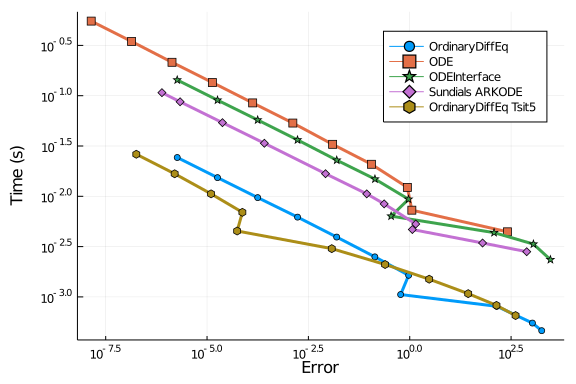
\includegraphics[width=\linewidth]{C:/Users/Chris/.julia/dev/DiffEqBenchmarks/NonStiffODE/jl_79E1.tmp/linear_wpd_2_1.pdf}

OrdinaryDiffEq.jl is clearly far in the lead, being more than an order of magnitude faster for the same amount of error.

\subsubsection{Full Saving}

\begin{lstlisting}
(*@\HLJLn{setups}@*) (*@\HLJLoB{=}@*) (*@\HLJLp{[}@*)(*@\HLJLnf{Dict}@*)(*@\HLJLp{(}@*)(*@\HLJLsc{:alg}@*)(*@\HLJLoB{=>}@*)(*@\HLJLnf{DP5}@*)(*@\HLJLp{(),}@*)(*@\HLJLoB{:}@*)(*@\HLJLn{dense}@*)(*@\HLJLoB{=>}@*)(*@\HLJLkc{false}@*)(*@\HLJLp{)}@*)
          (*@\HLJLnf{Dict}@*)(*@\HLJLp{(}@*)(*@\HLJLsc{:alg}@*)(*@\HLJLoB{=>}@*)(*@\HLJLnf{ode45}@*)(*@\HLJLp{(),}@*)(*@\HLJLoB{:}@*)(*@\HLJLn{dense}@*)(*@\HLJLoB{=>}@*)(*@\HLJLkc{false}@*)(*@\HLJLp{)}@*)
          (*@\HLJLnf{Dict}@*)(*@\HLJLp{(}@*)(*@\HLJLsc{:alg}@*)(*@\HLJLoB{=>}@*)(*@\HLJLnf{dopri5}@*)(*@\HLJLp{())}@*) (*@\HLJLcs{{\#} dense=false by default: no nonlinear interpolation}@*)
          (*@\HLJLnf{Dict}@*)(*@\HLJLp{(}@*)(*@\HLJLsc{:alg}@*)(*@\HLJLoB{=>}@*)(*@\HLJLnf{ARKODE}@*)(*@\HLJLp{(}@*)(*@\HLJLn{Sundials}@*)(*@\HLJLoB{.}@*)(*@\HLJLnf{Explicit}@*)(*@\HLJLp{(),}@*)(*@\HLJLn{etable}@*)(*@\HLJLoB{=}@*)(*@\HLJLn{Sundials}@*)(*@\HLJLoB{.}@*)(*@\HLJLn{DORMAND{\_}PRINCE{\_}7{\_}4{\_}5}@*)(*@\HLJLp{),}@*)(*@\HLJLoB{:}@*)(*@\HLJLn{dense}@*)(*@\HLJLoB{=>}@*)(*@\HLJLkc{false}@*)(*@\HLJLp{)}@*)
          (*@\HLJLnf{Dict}@*)(*@\HLJLp{(}@*)(*@\HLJLsc{:alg}@*)(*@\HLJLoB{=>}@*)(*@\HLJLnf{Tsit5}@*)(*@\HLJLp{(),}@*)(*@\HLJLoB{:}@*)(*@\HLJLn{dense}@*)(*@\HLJLoB{=>}@*)(*@\HLJLkc{false}@*)(*@\HLJLp{)]}@*)
(*@\HLJLn{names}@*) (*@\HLJLoB{=}@*) (*@\HLJLp{[}@*)(*@\HLJLs{"OrdinaryDiffEq"}@*)(*@\HLJLp{;}@*)(*@\HLJLs{"ODE"}@*)(*@\HLJLp{;}@*)(*@\HLJLs{"ODEInterface"}@*)(*@\HLJLp{;}@*)(*@\HLJLs{"Sundials ARKODE"}@*)(*@\HLJLp{;}@*)(*@\HLJLs{"OrdinaryDiffEq Tsit5"}@*)(*@\HLJLp{]}@*)
(*@\HLJLn{wp}@*) (*@\HLJLoB{=}@*) (*@\HLJLnf{WorkPrecisionSet}@*)(*@\HLJLp{(}@*)(*@\HLJLn{prob}@*)(*@\HLJLp{,}@*)(*@\HLJLn{abstols}@*)(*@\HLJLp{,}@*)(*@\HLJLn{reltols}@*)(*@\HLJLp{,}@*)(*@\HLJLn{setups}@*)(*@\HLJLp{;}@*)(*@\HLJLn{names}@*)(*@\HLJLoB{=}@*)(*@\HLJLn{names}@*)(*@\HLJLp{)}@*)
(*@\HLJLnf{plot}@*)(*@\HLJLp{(}@*)(*@\HLJLn{wp}@*)(*@\HLJLp{)}@*)
\end{lstlisting}

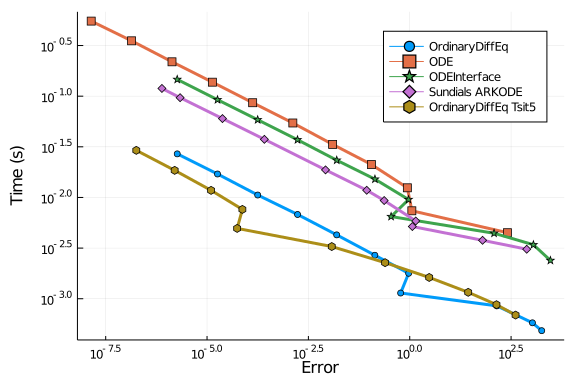
\includegraphics[width=\linewidth]{C:/Users/Chris/.julia/dev/DiffEqBenchmarks/NonStiffODE/jl_79E1.tmp/linear_wpd_3_1.pdf}

While not as dramatic as before, DifferentialEquations.jl is still far in the lead. Since the times are log scaled, this comes out to be almost a 5x lead over ODEInterface, and about a 10x lead over ODE.jl at default tolerances.

\subsubsection{Continuous Output}
Now we include continuous output. This has a large overhead because at every timepoint the matrix of rates \texttt{k} has to be deep copied.


\begin{lstlisting}
(*@\HLJLn{setups}@*) (*@\HLJLoB{=}@*) (*@\HLJLp{[}@*)(*@\HLJLnf{Dict}@*)(*@\HLJLp{(}@*)(*@\HLJLsc{:alg}@*)(*@\HLJLoB{=>}@*)(*@\HLJLnf{DP5}@*)(*@\HLJLp{())}@*)
          (*@\HLJLnf{Dict}@*)(*@\HLJLp{(}@*)(*@\HLJLsc{:alg}@*)(*@\HLJLoB{=>}@*)(*@\HLJLnf{ode45}@*)(*@\HLJLp{())}@*)
          (*@\HLJLnf{Dict}@*)(*@\HLJLp{(}@*)(*@\HLJLsc{:alg}@*)(*@\HLJLoB{=>}@*)(*@\HLJLnf{dopri5}@*)(*@\HLJLp{())}@*)
          (*@\HLJLnf{Dict}@*)(*@\HLJLp{(}@*)(*@\HLJLsc{:alg}@*)(*@\HLJLoB{=>}@*)(*@\HLJLnf{ARKODE}@*)(*@\HLJLp{(}@*)(*@\HLJLn{Sundials}@*)(*@\HLJLoB{.}@*)(*@\HLJLnf{Explicit}@*)(*@\HLJLp{(),}@*)(*@\HLJLn{etable}@*)(*@\HLJLoB{=}@*)(*@\HLJLn{Sundials}@*)(*@\HLJLoB{.}@*)(*@\HLJLn{DORMAND{\_}PRINCE{\_}7{\_}4{\_}5}@*)(*@\HLJLp{),}@*)(*@\HLJLoB{:}@*)(*@\HLJLn{dense}@*)(*@\HLJLoB{=>}@*)(*@\HLJLkc{false}@*)(*@\HLJLp{)}@*)
          (*@\HLJLnf{Dict}@*)(*@\HLJLp{(}@*)(*@\HLJLsc{:alg}@*)(*@\HLJLoB{=>}@*)(*@\HLJLnf{Tsit5}@*)(*@\HLJLp{())]}@*)
(*@\HLJLn{names}@*) (*@\HLJLoB{=}@*) (*@\HLJLp{[}@*)(*@\HLJLs{"OrdinaryDiffEq"}@*)(*@\HLJLp{;}@*)(*@\HLJLs{"ODE"}@*)(*@\HLJLp{;}@*)(*@\HLJLs{"ODEInterface"}@*)(*@\HLJLp{;}@*)(*@\HLJLs{"Sundials ARKODE"}@*)(*@\HLJLp{;}@*)(*@\HLJLs{"OrdinaryDiffEq Tsit5"}@*)(*@\HLJLp{]}@*)
(*@\HLJLn{wp}@*) (*@\HLJLoB{=}@*) (*@\HLJLnf{WorkPrecisionSet}@*)(*@\HLJLp{(}@*)(*@\HLJLn{prob}@*)(*@\HLJLp{,}@*)(*@\HLJLn{abstols}@*)(*@\HLJLp{,}@*)(*@\HLJLn{reltols}@*)(*@\HLJLp{,}@*)(*@\HLJLn{setups}@*)(*@\HLJLp{;}@*)(*@\HLJLn{names}@*)(*@\HLJLoB{=}@*)(*@\HLJLn{names}@*)(*@\HLJLp{)}@*)
(*@\HLJLnf{plot}@*)(*@\HLJLp{(}@*)(*@\HLJLn{wp}@*)(*@\HLJLp{)}@*)
\end{lstlisting}

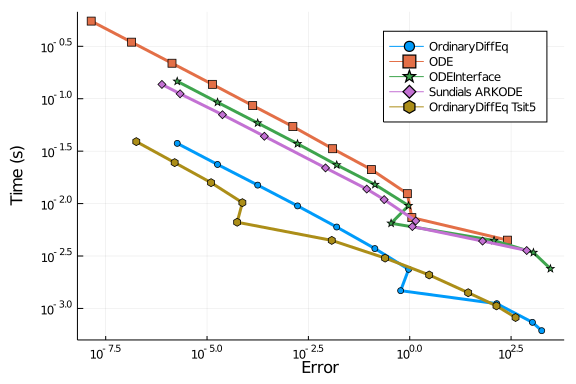
\includegraphics[width=\linewidth]{C:/Users/Chris/.julia/dev/DiffEqBenchmarks/NonStiffODE/jl_79E1.tmp/linear_wpd_4_1.pdf}

As you can see, even with this large overhead, DifferentialEquations.jl essentially ties with ODEInterface. This shows that the fully featured \texttt{DP5} solver holds its own with even the classic "great" methods.

\subsubsection{Other Runge-Kutta Algorithms}
Now let's test it against a smattering of other Runge-Kutta algorithms. First we will test it with all overheads off. Let's do the Order 5 (and the 2/3 pair) algorithms:


\begin{lstlisting}
(*@\HLJLn{setups}@*) (*@\HLJLoB{=}@*) (*@\HLJLp{[}@*)(*@\HLJLnf{Dict}@*)(*@\HLJLp{(}@*)(*@\HLJLsc{:alg}@*)(*@\HLJLoB{=>}@*)(*@\HLJLnf{DP5}@*)(*@\HLJLp{())}@*)
          (*@\HLJLnf{Dict}@*)(*@\HLJLp{(}@*)(*@\HLJLsc{:alg}@*)(*@\HLJLoB{=>}@*)(*@\HLJLnf{BS3}@*)(*@\HLJLp{())}@*)
          (*@\HLJLnf{Dict}@*)(*@\HLJLp{(}@*)(*@\HLJLsc{:alg}@*)(*@\HLJLoB{=>}@*)(*@\HLJLnf{BS5}@*)(*@\HLJLp{())}@*)
          (*@\HLJLnf{Dict}@*)(*@\HLJLp{(}@*)(*@\HLJLsc{:alg}@*)(*@\HLJLoB{=>}@*)(*@\HLJLnf{Tsit5}@*)(*@\HLJLp{())]}@*)
(*@\HLJLn{wp}@*) (*@\HLJLoB{=}@*) (*@\HLJLnf{WorkPrecisionSet}@*)(*@\HLJLp{(}@*)(*@\HLJLn{prob}@*)(*@\HLJLp{,}@*)(*@\HLJLn{abstols}@*)(*@\HLJLp{,}@*)(*@\HLJLn{reltols}@*)(*@\HLJLp{,}@*)(*@\HLJLn{setups}@*)(*@\HLJLp{;}@*)(*@\HLJLn{save{\_}everystep}@*)(*@\HLJLoB{=}@*)(*@\HLJLkc{false}@*)(*@\HLJLp{)}@*)
(*@\HLJLnf{plot}@*)(*@\HLJLp{(}@*)(*@\HLJLn{wp}@*)(*@\HLJLp{)}@*)
\end{lstlisting}

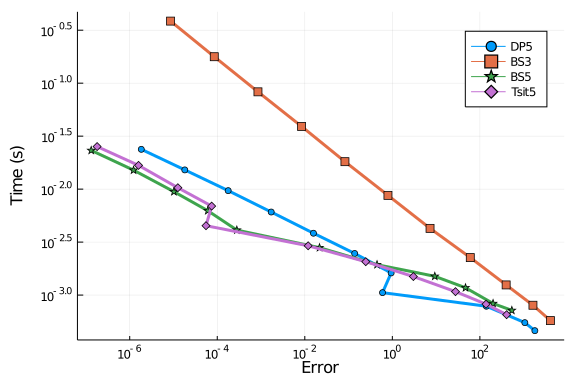
\includegraphics[width=\linewidth]{C:/Users/Chris/.julia/dev/DiffEqBenchmarks/NonStiffODE/jl_79E1.tmp/linear_wpd_5_1.pdf}

As you can see, the \texttt{Tsit5} algorithm is the most efficient, beating \texttt{DP5} which is more efficient than the Bogacki-Shampine algorithms. However, you can see that when the tolerance is high, \texttt{BS3} could be of use since its slope is so steep.

\subsection{Higher Order}
Now let's see how OrdinaryDiffEq.jl fairs with some higher order algorithms:


\begin{lstlisting}
(*@\HLJLn{setups}@*) (*@\HLJLoB{=}@*) (*@\HLJLp{[}@*)(*@\HLJLnf{Dict}@*)(*@\HLJLp{(}@*)(*@\HLJLsc{:alg}@*)(*@\HLJLoB{=>}@*)(*@\HLJLnf{DP5}@*)(*@\HLJLp{())}@*)
          (*@\HLJLnf{Dict}@*)(*@\HLJLp{(}@*)(*@\HLJLsc{:alg}@*)(*@\HLJLoB{=>}@*)(*@\HLJLnf{Vern6}@*)(*@\HLJLp{())}@*)
          (*@\HLJLnf{Dict}@*)(*@\HLJLp{(}@*)(*@\HLJLsc{:alg}@*)(*@\HLJLoB{=>}@*)(*@\HLJLnf{TanYam7}@*)(*@\HLJLp{())}@*)
          (*@\HLJLnf{Dict}@*)(*@\HLJLp{(}@*)(*@\HLJLsc{:alg}@*)(*@\HLJLoB{=>}@*)(*@\HLJLnf{Vern7}@*)(*@\HLJLp{())}@*)
          (*@\HLJLnf{Dict}@*)(*@\HLJLp{(}@*)(*@\HLJLsc{:alg}@*)(*@\HLJLoB{=>}@*)(*@\HLJLnf{Vern8}@*)(*@\HLJLp{())}@*)
          (*@\HLJLnf{Dict}@*)(*@\HLJLp{(}@*)(*@\HLJLsc{:alg}@*)(*@\HLJLoB{=>}@*)(*@\HLJLnf{DP8}@*)(*@\HLJLp{())}@*)
          (*@\HLJLnf{Dict}@*)(*@\HLJLp{(}@*)(*@\HLJLsc{:alg}@*)(*@\HLJLoB{=>}@*)(*@\HLJLnf{Vern9}@*)(*@\HLJLp{())]}@*)
(*@\HLJLn{wp}@*) (*@\HLJLoB{=}@*) (*@\HLJLnf{WorkPrecisionSet}@*)(*@\HLJLp{(}@*)(*@\HLJLn{prob}@*)(*@\HLJLp{,}@*)(*@\HLJLn{abstols}@*)(*@\HLJLp{,}@*)(*@\HLJLn{reltols}@*)(*@\HLJLp{,}@*)(*@\HLJLn{setups}@*)(*@\HLJLp{;}@*)(*@\HLJLn{save{\_}everystep}@*)(*@\HLJLoB{=}@*)(*@\HLJLkc{false}@*)(*@\HLJLp{)}@*)
(*@\HLJLnf{plot}@*)(*@\HLJLp{(}@*)(*@\HLJLn{wp}@*)(*@\HLJLp{)}@*)
\end{lstlisting}

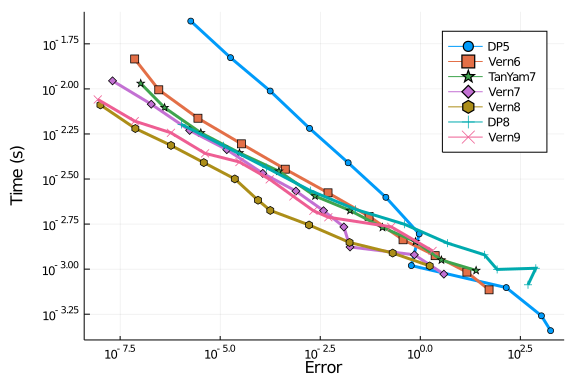
\includegraphics[width=\linewidth]{C:/Users/Chris/.julia/dev/DiffEqBenchmarks/NonStiffODE/jl_79E1.tmp/linear_wpd_6_1.pdf}

Vern7 looks to be the winner here, with DP5 doing well at higher tolerances but trailing of when it gets lower as one would expect with lower order algorithms. Some of the higher order methods, such as \texttt{Vern9}, would do better at lower tolerances than what's tested (outside of floating point range).

\subsection{Higher Order With Many Packages}
Now we test OrdinaryDiffEq against the high order methods of the other packages:


\begin{lstlisting}
(*@\HLJLk{using}@*) (*@\HLJLn{LSODA}@*)
(*@\HLJLn{setups}@*) (*@\HLJLoB{=}@*) (*@\HLJLp{[}@*)(*@\HLJLnf{Dict}@*)(*@\HLJLp{(}@*)(*@\HLJLsc{:alg}@*)(*@\HLJLoB{=>}@*)(*@\HLJLnf{DP5}@*)(*@\HLJLp{())}@*)
          (*@\HLJLnf{Dict}@*)(*@\HLJLp{(}@*)(*@\HLJLsc{:alg}@*)(*@\HLJLoB{=>}@*)(*@\HLJLnf{Vern7}@*)(*@\HLJLp{())}@*)
          (*@\HLJLnf{Dict}@*)(*@\HLJLp{(}@*)(*@\HLJLsc{:alg}@*)(*@\HLJLoB{=>}@*)(*@\HLJLnf{dop853}@*)(*@\HLJLp{())}@*)
          (*@\HLJLnf{Dict}@*)(*@\HLJLp{(}@*)(*@\HLJLsc{:alg}@*)(*@\HLJLoB{=>}@*)(*@\HLJLnf{ode78}@*)(*@\HLJLp{())}@*)
          (*@\HLJLnf{Dict}@*)(*@\HLJLp{(}@*)(*@\HLJLsc{:alg}@*)(*@\HLJLoB{=>}@*)(*@\HLJLnf{odex}@*)(*@\HLJLp{())}@*)
          (*@\HLJLnf{Dict}@*)(*@\HLJLp{(}@*)(*@\HLJLsc{:alg}@*)(*@\HLJLoB{=>}@*)(*@\HLJLnf{lsoda}@*)(*@\HLJLp{())}@*)
          (*@\HLJLnf{Dict}@*)(*@\HLJLp{(}@*)(*@\HLJLsc{:alg}@*)(*@\HLJLoB{=>}@*)(*@\HLJLnf{ddeabm}@*)(*@\HLJLp{())}@*)
          (*@\HLJLnf{Dict}@*)(*@\HLJLp{(}@*)(*@\HLJLsc{:alg}@*)(*@\HLJLoB{=>}@*)(*@\HLJLnf{ARKODE}@*)(*@\HLJLp{(}@*)(*@\HLJLn{Sundials}@*)(*@\HLJLoB{.}@*)(*@\HLJLnf{Explicit}@*)(*@\HLJLp{(),}@*)(*@\HLJLn{order}@*)(*@\HLJLoB{=}@*)(*@\HLJLni{8}@*)(*@\HLJLp{))}@*)
          (*@\HLJLnf{Dict}@*)(*@\HLJLp{(}@*)(*@\HLJLsc{:alg}@*)(*@\HLJLoB{=>}@*)(*@\HLJLnf{CVODE{\_}Adams}@*)(*@\HLJLp{())]}@*)
(*@\HLJLn{wp}@*) (*@\HLJLoB{=}@*) (*@\HLJLnf{WorkPrecisionSet}@*)(*@\HLJLp{(}@*)(*@\HLJLn{prob}@*)(*@\HLJLp{,}@*)(*@\HLJLn{abstols}@*)(*@\HLJLp{,}@*)(*@\HLJLn{reltols}@*)(*@\HLJLp{,}@*)(*@\HLJLn{setups}@*)(*@\HLJLp{;}@*)(*@\HLJLn{save{\_}everystep}@*)(*@\HLJLoB{=}@*)(*@\HLJLkc{false}@*)(*@\HLJLp{)}@*)
(*@\HLJLnf{plot}@*)(*@\HLJLp{(}@*)(*@\HLJLn{wp}@*)(*@\HLJLp{)}@*)
\end{lstlisting}

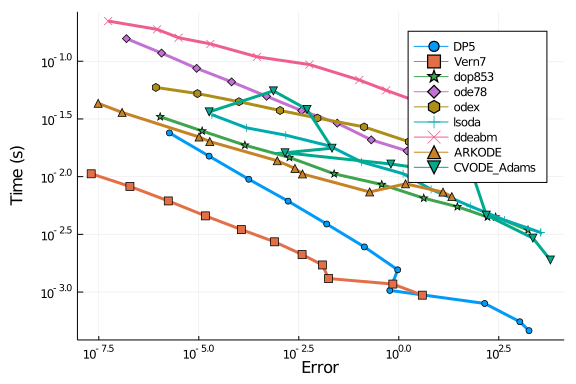
\includegraphics[width=\linewidth]{C:/Users/Chris/.julia/dev/DiffEqBenchmarks/NonStiffODE/jl_79E1.tmp/linear_wpd_7_1.pdf}

Here you can once again see the DifferentialEquations algorithms far in the lead. It's well known that for cheap function costs Adams methods are inefficient. ODE.jl one again has a bad showing.

\subsection{Interpolation Error}
Now we will look at the error using an interpolation measurement instead of at the timestepping points. Since the DifferentialEquations.jl algorithms have higher order interpolants than the ODE.jl algorithms, one would expect this would magnify the difference. First the order 4/5 comparison:


\begin{lstlisting}
(*@\HLJLn{setups}@*) (*@\HLJLoB{=}@*) (*@\HLJLp{[}@*)(*@\HLJLnf{Dict}@*)(*@\HLJLp{(}@*)(*@\HLJLsc{:alg}@*)(*@\HLJLoB{=>}@*)(*@\HLJLnf{DP5}@*)(*@\HLJLp{())}@*)
          (*@\HLJLcs{{\#}Dict(:alg=>ode45())}@*)
          (*@\HLJLnf{Dict}@*)(*@\HLJLp{(}@*)(*@\HLJLsc{:alg}@*)(*@\HLJLoB{=>}@*)(*@\HLJLnf{Tsit5}@*)(*@\HLJLp{())]}@*)
(*@\HLJLn{wp}@*) (*@\HLJLoB{=}@*) (*@\HLJLnf{WorkPrecisionSet}@*)(*@\HLJLp{(}@*)(*@\HLJLn{prob}@*)(*@\HLJLp{,}@*)(*@\HLJLn{abstols}@*)(*@\HLJLp{,}@*)(*@\HLJLn{reltols}@*)(*@\HLJLp{,}@*)(*@\HLJLn{setups}@*)(*@\HLJLp{;}@*)(*@\HLJLn{error{\_}estimate}@*)(*@\HLJLoB{=:}@*)(*@\HLJLn{L2}@*)(*@\HLJLp{,}@*)(*@\HLJLn{dense{\_}errors}@*)(*@\HLJLoB{=}@*)(*@\HLJLkc{true}@*)(*@\HLJLp{)}@*)
(*@\HLJLnf{plot}@*)(*@\HLJLp{(}@*)(*@\HLJLn{wp}@*)(*@\HLJLp{)}@*)
\end{lstlisting}

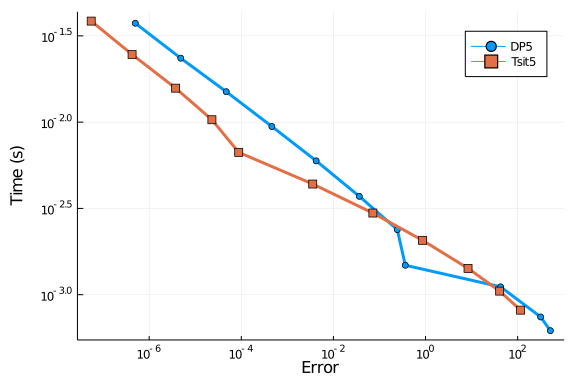
\includegraphics[width=\linewidth]{C:/Users/Chris/.julia/dev/DiffEqBenchmarks/NonStiffODE/jl_79E1.tmp/linear_wpd_8_1.pdf}

Note that all of ODE.jl uses a 3rd order Hermite interpolation, while the DifferentialEquations algorithms interpolations which are specialized to the algorithm. For example, \texttt{DP5} and \texttt{Tsit5} both use "free" order 4 interpolations, which are both as fast as the Hermite interpolation while achieving far less error. At higher order:


\begin{lstlisting}
(*@\HLJLn{setups}@*) (*@\HLJLoB{=}@*) (*@\HLJLp{[}@*)(*@\HLJLnf{Dict}@*)(*@\HLJLp{(}@*)(*@\HLJLsc{:alg}@*)(*@\HLJLoB{=>}@*)(*@\HLJLnf{DP5}@*)(*@\HLJLp{())}@*)
          (*@\HLJLnf{Dict}@*)(*@\HLJLp{(}@*)(*@\HLJLsc{:alg}@*)(*@\HLJLoB{=>}@*)(*@\HLJLnf{Vern7}@*)(*@\HLJLp{())}@*)
          (*@\HLJLcs{{\#}Dict(:alg=>ode78())}@*)
          (*@\HLJLp{]}@*)
(*@\HLJLn{wp}@*) (*@\HLJLoB{=}@*) (*@\HLJLnf{WorkPrecisionSet}@*)(*@\HLJLp{(}@*)(*@\HLJLn{prob}@*)(*@\HLJLp{,}@*)(*@\HLJLn{abstols}@*)(*@\HLJLp{,}@*)(*@\HLJLn{reltols}@*)(*@\HLJLp{,}@*)(*@\HLJLn{setups}@*)(*@\HLJLp{;}@*)(*@\HLJLn{error{\_}estimate}@*)(*@\HLJLoB{=:}@*)(*@\HLJLn{L2}@*)(*@\HLJLp{,}@*)(*@\HLJLn{dense{\_}errors}@*)(*@\HLJLoB{=}@*)(*@\HLJLkc{true}@*)(*@\HLJLp{)}@*)
(*@\HLJLnf{plot}@*)(*@\HLJLp{(}@*)(*@\HLJLn{wp}@*)(*@\HLJLp{)}@*)
\end{lstlisting}

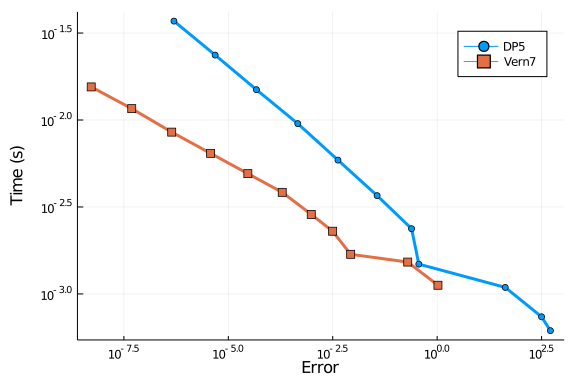
\includegraphics[width=\linewidth]{C:/Users/Chris/.julia/dev/DiffEqBenchmarks/NonStiffODE/jl_79E1.tmp/linear_wpd_9_1.pdf}

\subsection{Comparison with Fixed Timestep RK4}
Let's run the first benchmark but add some fixed timestep RK4 methods to see the difference:


\begin{lstlisting}
(*@\HLJLk{using}@*) (*@\HLJLn{GeometricIntegratorsDiffEq}@*)
\end{lstlisting}

\begin{lstlisting}
Error: ArgumentError: Package GeometricIntegratorsDiffEq not found in curre
nt path:
- Run `import Pkg; Pkg.add("GeometricIntegratorsDiffEq")` to install the Ge
ometricIntegratorsDiffEq package.
\end{lstlisting}


\begin{lstlisting}
(*@\HLJLn{abstols}@*) (*@\HLJLoB{=}@*) (*@\HLJLnfB{1.0}@*)(*@\HLJLoB{./}@*)(*@\HLJLnfB{10.0}@*)(*@\HLJLoB{.{\textasciicircum}}@*)(*@\HLJLp{(}@*)(*@\HLJLni{3}@*)(*@\HLJLoB{:}@*)(*@\HLJLni{13}@*)(*@\HLJLp{)}@*)
(*@\HLJLn{reltols}@*) (*@\HLJLoB{=}@*) (*@\HLJLnfB{1.0}@*)(*@\HLJLoB{./}@*)(*@\HLJLnfB{10.0}@*)(*@\HLJLoB{.{\textasciicircum}}@*)(*@\HLJLp{(}@*)(*@\HLJLni{0}@*)(*@\HLJLoB{:}@*)(*@\HLJLni{10}@*)(*@\HLJLp{);}@*)
(*@\HLJLn{dts}@*) (*@\HLJLoB{=}@*) (*@\HLJLp{[}@*)(*@\HLJLni{1}@*)(*@\HLJLp{,}@*)(*@\HLJLni{1}@*)(*@\HLJLoB{/}@*)(*@\HLJLni{2}@*)(*@\HLJLp{,}@*)(*@\HLJLni{1}@*)(*@\HLJLoB{/}@*)(*@\HLJLni{4}@*)(*@\HLJLp{,}@*)(*@\HLJLni{1}@*)(*@\HLJLoB{/}@*)(*@\HLJLni{10}@*)(*@\HLJLp{,}@*)(*@\HLJLni{1}@*)(*@\HLJLoB{/}@*)(*@\HLJLni{20}@*)(*@\HLJLp{,}@*)(*@\HLJLni{1}@*)(*@\HLJLoB{/}@*)(*@\HLJLni{40}@*)(*@\HLJLp{,}@*)(*@\HLJLni{1}@*)(*@\HLJLoB{/}@*)(*@\HLJLni{60}@*)(*@\HLJLp{,}@*)(*@\HLJLni{1}@*)(*@\HLJLoB{/}@*)(*@\HLJLni{80}@*)(*@\HLJLp{,}@*)(*@\HLJLni{1}@*)(*@\HLJLoB{/}@*)(*@\HLJLni{100}@*)(*@\HLJLp{,}@*)(*@\HLJLni{1}@*)(*@\HLJLoB{/}@*)(*@\HLJLni{140}@*)(*@\HLJLp{,}@*)(*@\HLJLni{1}@*)(*@\HLJLoB{/}@*)(*@\HLJLni{240}@*)(*@\HLJLp{]}@*)
(*@\HLJLn{setups}@*) (*@\HLJLoB{=}@*) (*@\HLJLp{[}@*)(*@\HLJLnf{Dict}@*)(*@\HLJLp{(}@*)(*@\HLJLsc{:alg}@*)(*@\HLJLoB{=>}@*)(*@\HLJLnf{DP5}@*)(*@\HLJLp{())}@*)
          (*@\HLJLnf{Dict}@*)(*@\HLJLp{(}@*)(*@\HLJLsc{:alg}@*)(*@\HLJLoB{=>}@*)(*@\HLJLnf{ode45}@*)(*@\HLJLp{())}@*)
          (*@\HLJLnf{Dict}@*)(*@\HLJLp{(}@*)(*@\HLJLsc{:alg}@*)(*@\HLJLoB{=>}@*)(*@\HLJLnf{dopri5}@*)(*@\HLJLp{())}@*)
          (*@\HLJLnf{Dict}@*)(*@\HLJLp{(}@*)(*@\HLJLsc{:alg}@*)(*@\HLJLoB{=>}@*)(*@\HLJLnf{GIERK4}@*)(*@\HLJLp{(),}@*)(*@\HLJLoB{:}@*)(*@\HLJLn{dts}@*)(*@\HLJLoB{=>}@*)(*@\HLJLn{dts}@*)(*@\HLJLp{)}@*)
          (*@\HLJLnf{Dict}@*)(*@\HLJLp{(}@*)(*@\HLJLsc{:alg}@*)(*@\HLJLoB{=>}@*)(*@\HLJLnf{RK4}@*)(*@\HLJLp{(),}@*)(*@\HLJLoB{:}@*)(*@\HLJLn{dts}@*)(*@\HLJLoB{=>}@*)(*@\HLJLn{dts}@*)(*@\HLJLp{)}@*)
          (*@\HLJLnf{Dict}@*)(*@\HLJLp{(}@*)(*@\HLJLsc{:alg}@*)(*@\HLJLoB{=>}@*)(*@\HLJLnf{Tsit5}@*)(*@\HLJLp{())]}@*)
\end{lstlisting}

\begin{lstlisting}
Error: UndefVarError: GIERK4 not defined
\end{lstlisting}


\begin{lstlisting}
(*@\HLJLn{names}@*) (*@\HLJLoB{=}@*) (*@\HLJLp{[}@*)(*@\HLJLs{"DifferentialEquations"}@*)(*@\HLJLp{;}@*)(*@\HLJLs{"ODE"}@*)(*@\HLJLp{;}@*)(*@\HLJLs{"ODEInterface"}@*)(*@\HLJLp{;}@*)(*@\HLJLs{"GeometricIntegrators RK4"}@*)(*@\HLJLp{;}@*)(*@\HLJLs{"DifferentialEquations RK4"}@*)(*@\HLJLp{;}@*)(*@\HLJLs{"DifferentialEquations Tsit5"}@*)(*@\HLJLp{]}@*)
(*@\HLJLn{wp}@*) (*@\HLJLoB{=}@*) (*@\HLJLnf{WorkPrecisionSet}@*)(*@\HLJLp{(}@*)(*@\HLJLn{prob}@*)(*@\HLJLp{,}@*)(*@\HLJLn{abstols}@*)(*@\HLJLp{,}@*)(*@\HLJLn{reltols}@*)(*@\HLJLp{,}@*)(*@\HLJLn{setups}@*)(*@\HLJLp{;}@*)(*@\HLJLn{names}@*)(*@\HLJLoB{=}@*)(*@\HLJLn{names}@*)(*@\HLJLp{,}@*)
                      (*@\HLJLn{save{\_}everystep}@*)(*@\HLJLoB{=}@*)(*@\HLJLkc{false}@*)(*@\HLJLp{,}@*)(*@\HLJLn{verbose}@*)(*@\HLJLoB{=}@*)(*@\HLJLkc{false}@*)(*@\HLJLp{)}@*)
(*@\HLJLnf{plot}@*)(*@\HLJLp{(}@*)(*@\HLJLn{wp}@*)(*@\HLJLp{)}@*)
\end{lstlisting}

\begin{lstlisting}
Error: DimensionMismatch("new dimensions (1, 2) must be consistent with arr
ay size 6")
\end{lstlisting}


\subsection{Conclusion}
DifferentialEquations's default choice of \texttt{Tsit5} does well for quick and easy solving at normal tolerances. However, at low tolerances the higher order algorithms are faster. In every case, the DifferentialEquations algorithms are far in the lead, many times an order of magnitude faster than the competitors. \texttt{Vern7} with its included 7th order interpolation looks to be a good workhorse for scientific computing in floating point range. These along with many other benchmarks are why these algorithms were chosen as part of the defaults.



\end{document}
